%\documentclass[12pt,a4paper,twoside,titlepage,headsepline,pointlessnumbers,liststotoc,idxtotoc,bibtotoc,ngerman]{scrartcl}
\documentclass[12pt,a4paper,twoside,titlepage,headsepline,pointlessnumbers,liststotoc,idxtotoc,bibtotoc,ngerman,english]{scrreprt}
%\documentclass[12pt,a4paper,twoside,titlepage,openright,headsepline,listof=totoc,index=totoc,chapterprefix,bibliography=totoc]{scrreprt}

\ifx\pdfoutput\undefined
\pdffalse % we are not running pdflatex
\else
\pdfoutput=1 % we are running pdflatex
\pdfcompresslevel=9     % compression level for text and image;
\usepackage[pdftex,bookmarks=true,bookmarksopen=false,bookmarksnumbered=true,linktocpage,colorlinks=true,backref,pagebackref, linkcolor=black,  citecolor=black, urlcolor=black]{hyperref}
\usepackage[pdftex]{graphicx}
\usepackage[final]{pdfpages}

% Setzt die Einrücktiefe der ersten Zeile nach einem Absatz auf 0
\setlength{\parindent}{0pt} 
\usepackage{needspace}


\usepackage{amsfonts}
\usepackage{algorithmic}
\usepackage{bibgerm}
\usepackage{url}
\usepackage{color}
\usepackage{tabularx}
\usepackage[T1]{fontenc} 
\usepackage[utf8]{inputenc}
\usepackage{bbm}
\usepackage{amsmath}
\usepackage{amssymb}
\usepackage{ntheorem}
\usepackage{fancyvrb}
\usepackage{subfigure}
%\usepackage{ngerman}
\usepackage[english]{babel}
\usepackage{mathptmx} 
\usepackage[scaled=.90]{helvet} 
\usepackage{courier}
\usepackage[rightcaption]{sidecap}
\usepackage{lscape}
\usepackage{supertabular} 
\usepackage{graphicx}
\usepackage{tabularx}

% Listings
\usepackage{listings}
\lstset{basicstyle=\small,captionpos=b}

\newenvironment{packed_enum}{
\begin{enumerate}
  \setlength{\itemsep}{0.5pt}
  \setlength{\parskip}{0pt}
  \setlength{\parsep}{0pt}
}{\end{enumerate}}

\RequirePackage{xspace}

\setcounter{secnumdepth}{3}
\selectlanguage{english} % Dokumentensprache auf englisch stellen
%\selectlanguage{german} % Dokumentensprache auf deutsch stellen


\newcommand{\p}[1]{\texttt{\small #1}}
\newcommand{\INFO}[1]{{\small~\\\hrule\vspace{0.1cm}\hrule~\\\textbf{Information:}\\#1~\\\hrule\vspace{0.1cm}\hrule~\\}}
%\theoremstyle{break}
%\newtheorem{defi}{Definition}[section] 
%\newtheorem{bsp}{Beispiel}[section] 

\definecolor{gray}{gray}{0.95}
\setlength{\fboxrule}{2pt}

\providecommand{\ext}[1]{}
\providecommand{\TODO}[1]{{\small ~\\\hrule\vspace{0.1cm}\hrule~\\\textbf{TODO}:  #1~\\\hrule\vspace{0.1cm}\hrule~\\}}

\pagestyle{headings}

\begin{document}                
             

	% ************************************************************
	% *****                    Titelseite                    *****
	% ************************************************************


	\setcounter{page}{1}
	\pagenumbering{Roman}

	\begin{titlepage}
	\thispagestyle{empty}
	\begin{center}

			
\includegraphics[width=12cm]{figures/Logo_Uni_Paderborn}\\
			\textsf{
			Fakultät für Elektrotechnik, Informatik und Mathematik \\
			Institut für Informatik, Fachgebiet Softwaretechnik \\ 
      		Warburger Straße 100 \\
			33098 Paderborn} \\
                    
      \vspace{4cm}									

			{\LARGE  \textbf{Tutorials}} \\ 
			\vspace{0.5cm}
			{\Large From the Fujaba context} \\ 
			\vspace{2.5cm}

			\vspace{0.5cm}
			\textbf{Author:} Ingo Budde \\
			\vspace{1cm}
			Paderborn, \today \\
			\vspace{1cm}
			
	\end{center}
	\end{titlepage}

	\clearpage
		
	\thispagestyle{empty}
	
	\tableofcontents
	
	\clearpage
  
  \pagenumbering{arabic}
	\setcounter{page}{1}

	\chapter{Fujaba Diagram Editors with GMF}
	
\section{Overview}
\subsection{Introduction}
In this document several solutions will be provided that help developing a
GMF-Diagram Editor for Fujaba.
It is not necessary to do it exactly this way, but it should give the reader a
good orientation.

\subsection{Multiple ways of modifying the generated editor}
Basically there are multiple ways to modify the look and behavior of the
generated editor.
\begin{enumerate}
    \item Adjusting the generated code directly (myeditor.diagram)
	\item Creation of a "Extension"-Plugin (myeditor.diagram.custom)
\end{enumerate}

In this document, the second variant will be chosen, so that the GMF-Code can be
regenerated without problems. Furthermore, this way there is a strict separation
of generated and manually written sourcecode. This idea was taken from Dr. Köhnlein's
\href{http://www.slideshare.net/itemis/gmf-fr-anspruchsvolle-presentation}{slides}
at w-jax08 (slides 20-22). \\
In case, changes on the generated code are unavoidable, this can be achieved by
modifying the gmf-templates used to generate the code.

\subsection{Conventions}
It is assumed that the editor is called MyEditor. 

\section {Creating a NewWizard for a Fujaba Diagram Editor}
Fujaba Diagram Editor share a domain model file (the fujaba model).
Therefore a New Wizard for Fujaba Diagrams must be able to put a new
diagram into an existing model file, without deleting all of its contents.
An abstract implementation for such a New Wizard exists within the
$de.uni\_paderborn.fujaba.newwizard$ plugin.

\subsection {MANIFEST.MF}
In order to use the abstract implementation, make sure that your
$myeditor.custom$ plugin has a dependency to
$de.uni\_paderborn.fujaba.newwizard$.

\subsection {plugin.xml}
\lstinputlisting
[caption={An extension must be added to the
plugin.xml}\label{lst:javaclass},language=XML]
{files/newwizard/plugin.xml}


\subsection {Class CustomMyEditorDiagramCreationWizard}
\lstinputlisting
[caption={Example for
myeditor.diagram.custom.part.MyEditorDiagramCreationWizard.}
\label{lst:javaclass},language=JAVA] {files/newwizard/newwizard.java}

	\chapter{Techreport Generator}
\section{Overview}
The Mechatronic UML Meta-Model is based on ecore, which supports annotation of
elements in order to add documentation.
Additionally the paper "Mechatronic UML Syntax and Semantics" explains many
design decisions and has a dedicated chapter, which covers the contents of the
Mechatronic UML Meta-Model.

To avoid the situation that both places contain redundant documentation and to
avoid resulting inconsistencies, it has been decided to use the Xpand
template language of the OpenArchitectureWare Project to derive documentation
annotations.

\section{How does it work?}
The Project GeneratorTechreport in the mumlpaper repository is a
OpenArchitectureWare Workflow.
It is able to access the Mechatronic UML Meta-Model ecore file, if the Meta
Model is checked out correctly as a seperate plugin.

It is supposed that the muml.ecore file is accessable in the following
location:\\
\textbf{/de.uni\_paderborn.fujaba.muml.model/model}
(relative to the workspace directory).

Additionally the following dependant ecore files must exist:
\begin{itemize}
  \item \textbf{/org.storydriven.modeling/model/sdm.ecore} and
  \item \textbf{/de.uni\_paderborn.fujaba.modelinstance/model/modelinstance.ecore}
\end{itemize}

Lastly the \textbf{Mechatronic UML Syntax and Semantics} Paper should be checked
out, because the Workflow generates into the following location:\\
\textbf{/MUML Syntax and Semantics/08\_TechDoc\_Contents.tex}.

\section{How to install OpenArchitectureWare?}
Our workflow depends on the (old) OpenArchitectureWare project, before it merged
into the Eclipse Modeling Project. The eclipse plugins can be downloaded from:\\
\href{http://www.openarchitectureware.org/staticpages/index.php/download}
{\textbf{http://www.openarchitectureware.org/staticpages/index.php/download}}
\\
I personally prefer using the update site, which is also stated on the
website.\\
\href{http://www.openarchitectureware.org/updatesite/milestone/site.xml}
{\textbf{http://www.openarchitectureware.org/updatesite/milestone/site.xml}}

\begin{figure}[htbp]
  \centering
  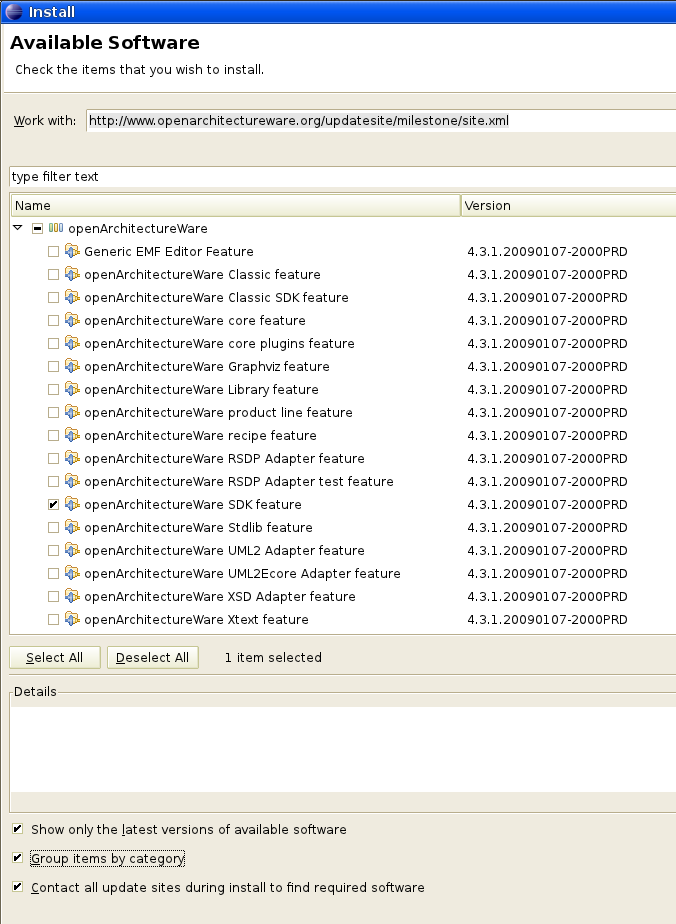
\includegraphics[width=0.5\linewidth]{figures/OAW-UpdateSite}
  \caption{Installing the OpenArchitectureWare Plugin using the Update Site}
\end{figure}

For our Generator Project it is sufficient to install the OpenArchitectureWare
SDK Feature.

\section{How to start the Workflow?}
After the installation has been completed, the workflow can be started by
right-clicking the \textbf{generateDoc.oaw} file in the folder

\textbf{src/workflow} and selecting \textbf{Run As$\to$ oAW Workflow}.

\begin{figure}[htbp]
  \centering
  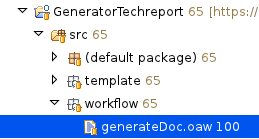
\includegraphics[width=0.5\linewidth]{figures/OAW-WorkflowFile}
  \caption{Selecting generateDoc.oaw}
\end{figure}

\begin{figure}[htbp]
  \centering
  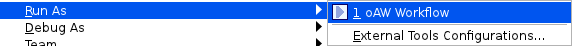
\includegraphics[width=1\linewidth]{figures/OAW-RunAs}
  \caption{Running the oAW-Workflow}
\end{figure}

\textbf{Note:} If you installed a newer version of OpenArchitectureWare than
used here, the context menu will only present you \textbf{Run As$\to$ MWE
Workflow} (Modeling Workflow Engine). This newer engine does not work with our
workflow.\\

\textbf{Note:} In the console view there might appear some warnings, which can
be ignored for now.
	

%	\listoffigures % Abbildungsverzeichnis

	% ************************************************************
	% *****                      Ende                        *****
	% ************************************************************

\end{document}